\section{Localization}
\label{sec::localisation}
Finally, a method to compute the state (configuration) of the robot is required. The method should be applied to a real system such as the Nexus platform from the course and due to the size of the university it is important that the robot is able to use features to precisely measure its whereabouts. These features could be based on the Hokoyo 2D laser scanner mounted on the robot.\\[0.2cm]
Again document what algorithm, and test how well it performs. You should at least write what model you choose for the robot and show that the localisation works better than odometry alone.\\[0.2cm]
In the real world, no actuator is perfect: they may overshoot or undershoot the desired amount of motion. So when a robot tries to drive in a straight line, it will inevitably curve to one side or the other due to minute differences in wheel radius. Figure \ref{fig::MC_test} shows how the position of a robot can get more and more uncertain, as it moves in straight lines. A robot becomes less sure of its position if it moves blindly without sensing the environment, so it is necessary to sensors to localize the robot in the environment, and not only count on the odometry alone. To solve this, on the robot is a 2D laser range scanner mounted to sense the environment around it.
\begin{figure}[H]
\centering
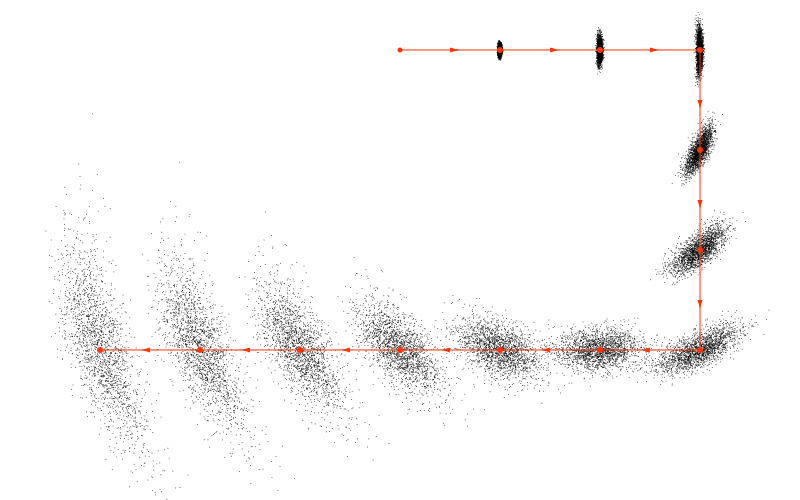
\includegraphics[scale=0.43]{img/MCtest.png}
\caption{Belief after moving several steps for a 2D robot using a typical motion model without sensing.}
\label{fig::MC_test}
\end{figure}
All localization is done online, and it involves the functions:
\begin{itemize}\itemsep-2pt
\item \textbf{Monte Carlo localization (MCL)} for determining the localization of the robot as it moves. This algorithm is normally used for robots to localize using a particle filter.
\item \textbf{Set linear speed} for the robot, to determine how fast it should move
\item \textbf{Set rotations speed} on each wheel of the robot, so it possible for it to turn 90 degrees to either left or right.  
\end{itemize}
\newpage
\subsection{Solution}
The MCL is given a map of the environment, and then the algorithm estimates the position and orientation of a robot as it moves and senses the environment. This is used to determine the position of the robot, by following\footnote{\url{http://en.wikipedia.org/wiki/Monte_Carlo_localization}} 
\begin{enumerate}\itemsep-2pt
\item The algorithm uses a particle filter to represent the distribution of likely states, with each particle representing a possible state, i.e. a hypothesis of where the robot is. First $N$ numbers of normal distributed hypothesis of the robots position is made of the entire map. At this point, the robot has no information about where it is and can only assumes it is equally likely to be at any point in configuration space.
\item All the hypothesis is compared to what the 2D laser range scanner sees, and that hypothesis with the highest probability, i.e. how well the actual sensed data correlate with the predicted position, an is assumed being the robots current position.
\item Whenever the robot moves, it shifts the particles to predict its new state after the movement, so, $N$ normal distributed hypotheses surrounding our current position--hypothesis is made within a smaller area around the predicted current position. Maintaining the entire map as sample size would be computationally wasteful and make the the calculations less precise.
\item Step 2 to 4 is repeated with the previous belief as input, because ultimately, the particles should converge towards the actual position of the robot. This is repeated until the robot is either turned off or done collecting the cups.
\end{enumerate}
Figure \ref{fig::MC} shows the implemented Monte Carlo method on the robot. The yellow dots are the hypothesis that is normal distributed around the robot and the red dot is the robots current position according to the hypothesis and what the 2D laser range scanner sees. All white pixels are free space and the black pixels are obstacles. The robot is seen as a point--robot in this example.\\[0.2cm]

\begin{figure}[H]
\centering
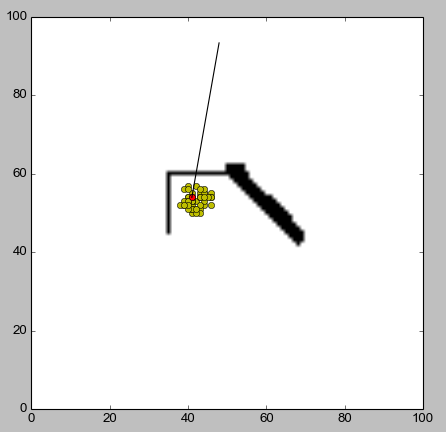
\includegraphics[scale=0.43]{img/MC.png}
\caption{Monte Carlo hypothesis (yellow dots) and the current position (red dot)}
\label{fig::MC}
\end{figure}

\newpage
\subsection{Results}
To test how accurately the implemented Monte Carlo method detects, where on the map the robot is located, a experimental setup for testing the robots real and virtual position is shown on figure \ref{fig::experimental}. On the figure, a construction similar to the map on figure \ref{fig::MC_test} is made and 10x10 cm is drawn on the floor. This indicates each pixel on the map and makes it possible to compare the current real position with the virtual position. 

\begin{figure}[H]
\centering 
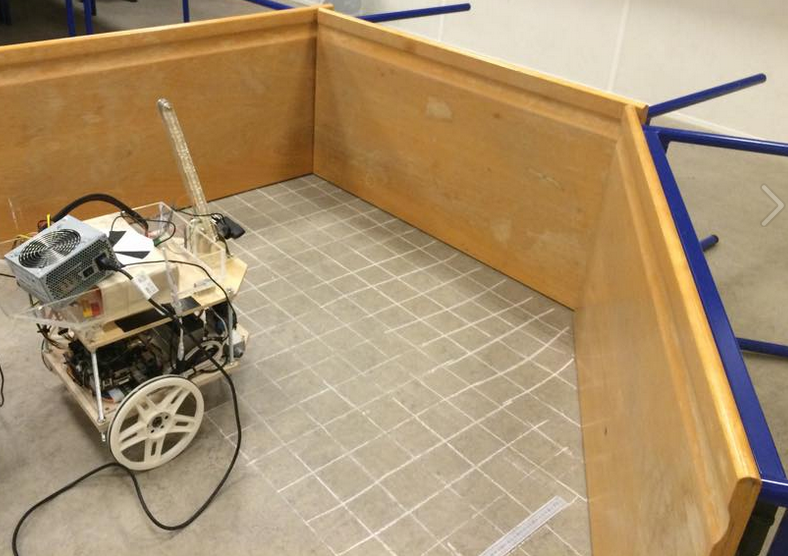
\includegraphics[scale=0.3]{img/test.png}
\caption{The experimental setup for testing the robots real and virtual position}
\label{fig::experimental}
\end{figure}

The steps for testing is done by the following steps
\begin{enumerate}\itemsep-2pt
\item The robot is moved to a position
\item The real and virtual position is noted
\item The real and virtual degree is noted
\end{enumerate}
The results is shown in table \ref{tab::results} and by look at the collected data, it can be seen that the virtual position correspond well to the real position.

\begin{table}[H]
\begin{tabular}{|lrlrll|lrlrl|}
\rowcolor[HTML]{9B9B9B} 
Mesurement 1            & pos x &         & pos y &    &  & Mesurement 4            & pos x   &         & posy  &    \\
Real position           & 39    & px      & 53    & px &  & Real position           & 47      & px      & 53    & px \\
Virtual position        & 39    & px      & 53    & px &  & Virtual position        & 39      & px      & 46    & px \\
Real $\theta$    & 0     & degrees &       &    &  & Real $\theta$    & 90      & degrees &       &    \\
Virtual $\theta$ & 0-12  & degrees &       &    &  & Virtual $\theta$ & 9-15    & degrees &       &    \\
                        &       &         &       &    &  &                         &         &         &       &    \\
\rowcolor[HTML]{9B9B9B} 
Mesurement 2            & pos x &         & pos y &    &  & Mesurement 5            & pos x   &         & pos y &    \\
Real position           & 42    & px      & 56    & px &  & Real position           & 48      & px      & 55    & px \\
Virtual position        & 43    & px      & 56    & px &  & Virtual position        & 51      & px      & 55    & px \\
Real $\theta$    & 0-12  & degrees &       &    &  & Real $\theta$   & 335     & degrees &       &    \\
Virtual $\theta$& 1-5   & degrees &       &    &  & Virtual $\theta$ & 328-331 & degrees &       &    \\
                        &       &         &       &    &  &                         &         &         &       &    \\
\rowcolor[HTML]{9B9B9B} 
Mesurement 3            & pos x &         & pos y &    &  & Mesurement 6            & pos x   &         & pos y &    \\
Real position           & 40    & px      & 56    & px &  & Real position           & 44      & px      & 51    & px \\
Virtual position        & 39    & px      & 56    & px &  & Virtual position        & 45      & px      & 51    & px \\
Real $\theta$    & 45    & degrees &       &    &  & Real $\theta$    & 0       & degrees &       &    \\
Virtual $\theta$ & 45-50 & degrees &       &    &  & Virtual $\theta$ & 5-10    & degrees &       &   \\ 
 &  &  &       &    &  &  &    &  &       &   \\ \hline
\end{tabular}
\caption{Results}
\label{tab::results}
\end{table}

\subsection{Alternatives}
As alternatives to localization could the following methods may also be used:
\begin{itemize}\itemsep-2pt
\item Kalman filter
\end{itemize}

